\section{Auswertung}
\label{sec:Auswertung}

\subsection{Überprüfung der Bragg-Bedingung}
\begin{figure}
	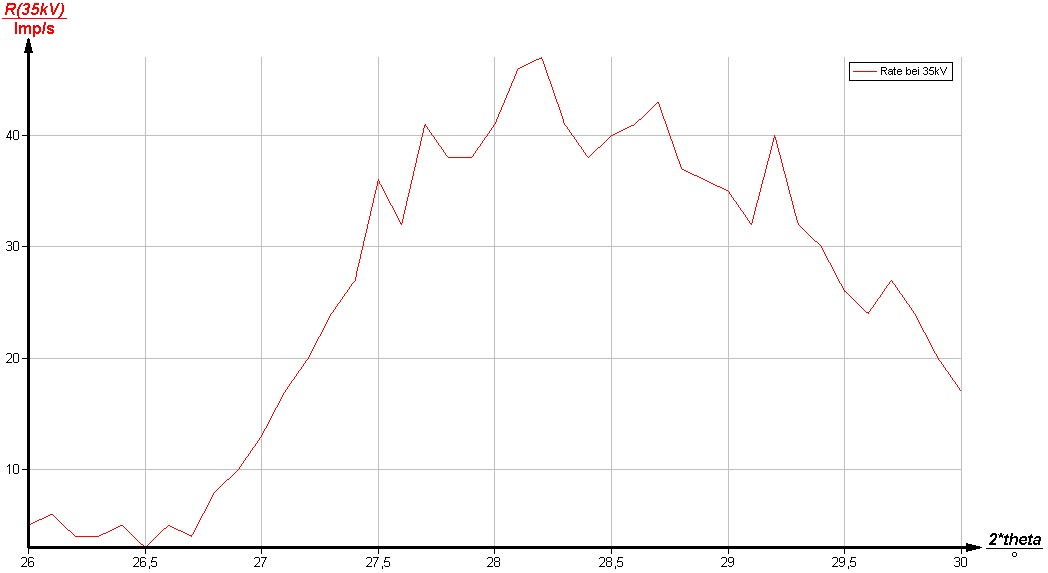
\includegraphics[width=1.0\textwidth]{nIKO_und_jULIAN_ÜLADS/breck.jpg}
	\caption{Gemessene Impulse in Abhängigkeit des abgelaufenen Winkels zur Überprüfung der Bragg-Bedingung.}
	\label{fig:Braggi}
\end{figure}
Zur Überprüfung der Bragg-Bedindung wird das Maximum der Messkurve in Plot \ref{fig:braeck} bestimmt.
Um das Maximum möglichst genau bestimmen zu können sind die von der Messapparatur aufgenommenen Messdaten um das Maximum herum in Tabelle \ref{tab:bregg} aufgetragen.
Das Maximum wird abgelesen zu $\theta=28.2$


\begin{table}
	\caption{title}
	\label{tab:bregg}
	\begin{tabular} {cc}
		$2 \cdot \theta$ /$\textdegree$ &Impulse \\%blaa angaben in grad?
		27,5	&36,0\\
		27,6	&32,0\\
		27,7	&41,0\\
		27,8	&38,0\\
		27,9	&38,0\\
		28,0	&41,0\\
		28,1	&46,0\\
		28,2	&47,0\\
		28,3	&41,0\\
		28,4	&38,0\\
		28,5	&40,0\\
		28,6	&41,0\\
		28,7	&43,0\\
		28,8	&37,0\\
	\end{tabular}
\end{table}

\subsection{Das Emissionsspektrum der Kupfer-Röntgenröhre}

\begin{figure}
	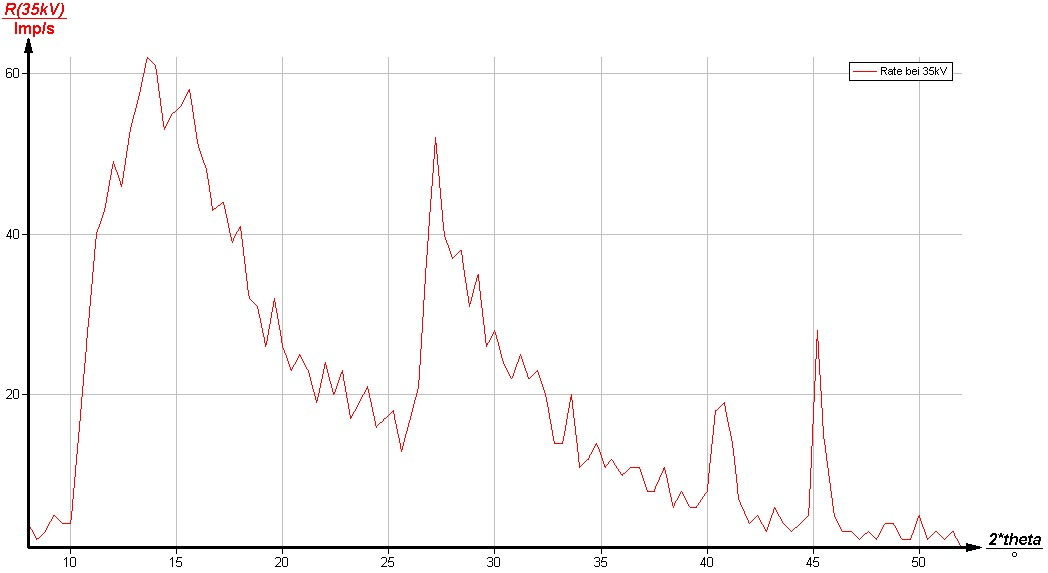
\includegraphics[width=1.0\textwidth]{nIKO_und_jULIAN_ÜLADS/Kupfaemmision.jpg}
	\caption{Aufgenommenes Emissionssspektrum der Kupfer-Röntgenröhre.}
	\label{fig:emissionlol}
\end{figure}




%%%%%%%%%%%%%%%%%%%%%%%%%%%%%%%%%%%%%%%%%%%%%%%%%%%%%%%%%%%%%%%%%%%%%%%%%%%%%%%%%%%%%%%%%%
\FloatBarrier
\subsection{Das Absorptionsspektrum}

\subsubsection{Absorber Zink}
\begin{figure}
	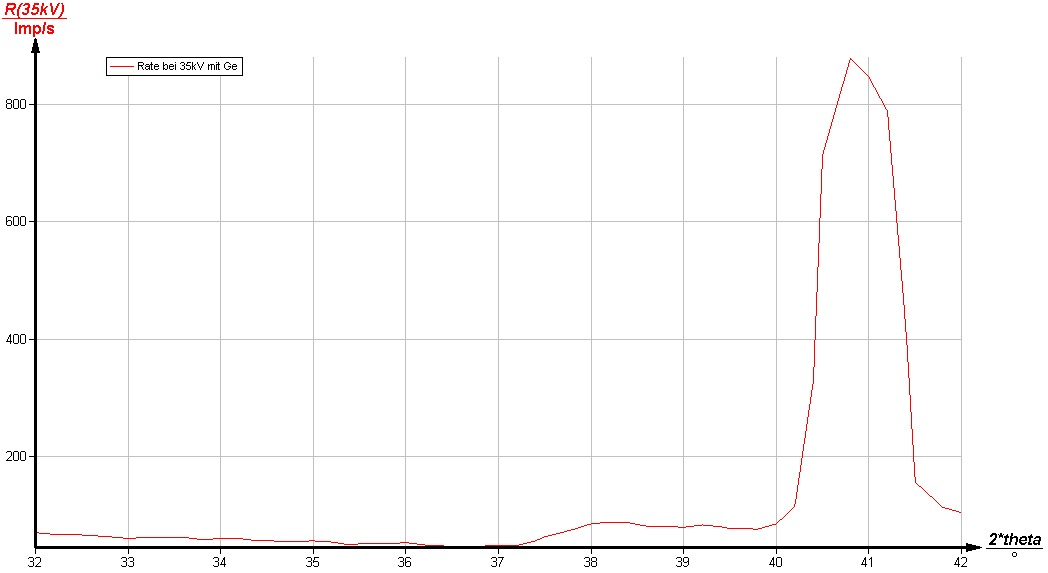
\includegraphics[width=1.0\textwidth]{nIKO_und_jULIAN_ÜLADS/zink.jpg}
	\caption{Aufgenommenes Absorptionsspektrum mit dem Absorber Zink.}
	\label{fig:zink_absorber}
\end{figure}
Mit Formel \eqref{eqn:braggii} und dem Zusammenhang $E = \frac{\symup{hc}}{\lambda}$,
wobei $\symup{h}$
das Planck'sche Wirkungsquantum und $\symup{c}$ die Lichtgeschwindigkeit im Vakuum ist, lässt
sich die Absorptionsenergie durch
\begin{equation}
	\label{eqn:Absorptionsenergie}
	E = \frac{\symup{hc}}{2d\sin\theta}
\end{equation}
ermitteln.

%%%%%%%%%%%%%%%%%%%%%%%%%%%%%%%%%%%%%%%%%%%%%%%%%%%%%
\FloatBarrier
\subsubsection{Absorber Germanium}
\begin{figure}
	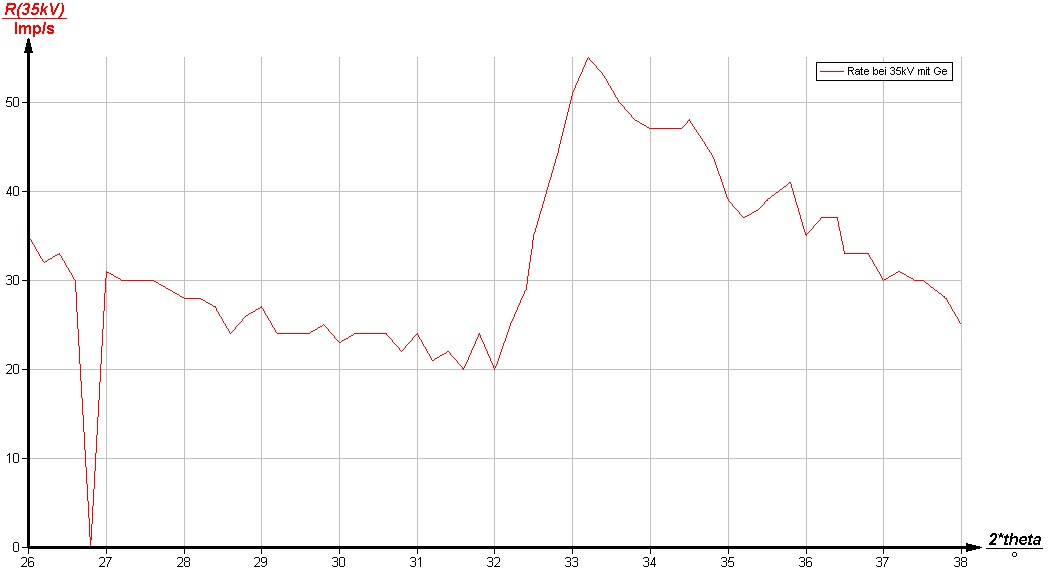
\includegraphics[width=1.0\textwidth]{nIKO_und_jULIAN_ÜLADS/germanium.jpg}
	\caption{Aufgenommenes Absorptionsspektrum mit dem Absorber Germanium.}
	\label{fig:germanium_absorber}
\end{figure}
Das Absorptionsspektrum von Germanium ist in Abbildung \ref{fig:germanium_absorber}
dargestellt. Es wird die K-Kante bei
\begin{equation*}
	\theta_{\mathrm{Ge,K}} = \SI{16,0}{\degree}
\end{equation*}
abgelesen. Damit ergibt sich nach Formel \eqref{eqn:Absorptionsenergie} die Absorptionsenergie
von Germanium zu
\begin{equation*}
	E_{\mathrm{Ge,K}} = -\SI{10.6912923(1)}{\kilo\electronvolt} \mathrm{.}
\end{equation*}
Weiterhin lässt sich mit Formel \eqref{eqn:} die Abschirmzahl von Germanium zu
\begin{equation*}
	\sigma_{\mathrm{Ge,K}} = 2
\end{equation*}
berechnen.

%%%%%%%%%%%%%%%%%%%%%%%%%%%%%%%%%%%%%%%%%%%%%%%%%%%%%%%%%
\FloatBarrier
\subsubsection{Absorber Brom}
\begin{figure}
	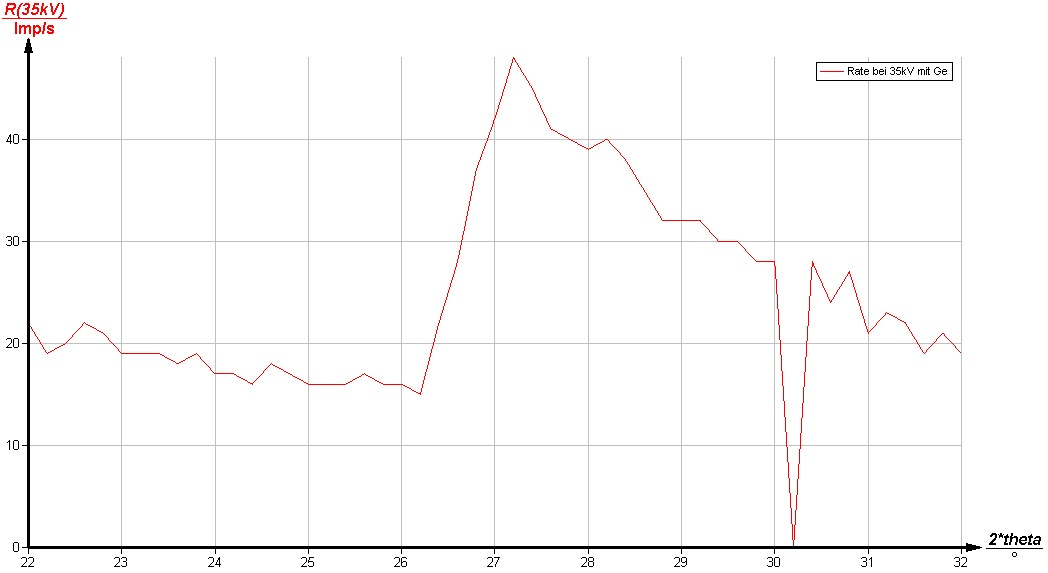
\includegraphics[width=1.0\textwidth]{nIKO_und_jULIAN_ÜLADS/brom.jpg}
	\caption{Aufgenommenes Absorptionsspektrum mit dem Absorber Brom.}
	\label{fig:brom_absorber}
\end{figure}

\FloatBarrier
\subsubsection{Absorber Zirkonium}
\begin{figure}
	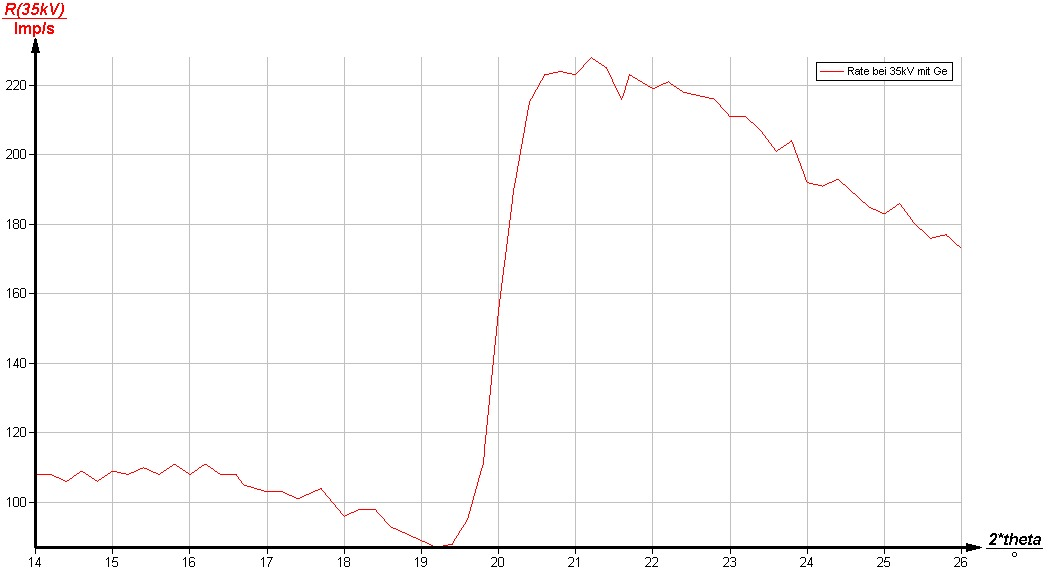
\includegraphics[width=1.0\textwidth]{nIKO_und_jULIAN_ÜLADS/zirkonium.jpg}
	\caption{Aufgenommenes Absorptionsspektrum mit dem Absorber Zirkonium.}
	\label{fig:zirkonium_absorber}
\end{figure}

\FloatBarrier
\subsubsection{Absorber Gold}
\begin{figure}
	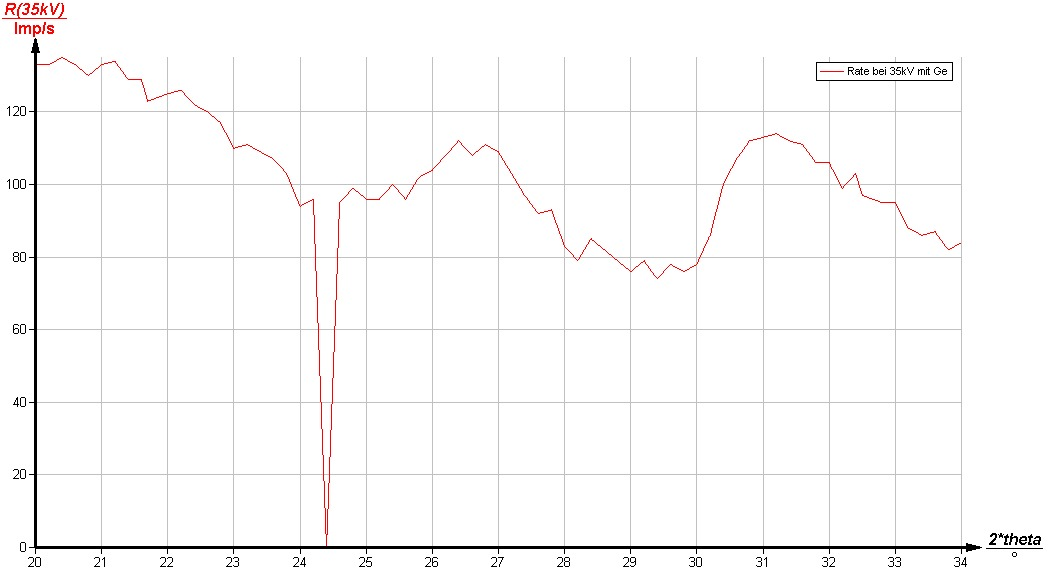
\includegraphics[width=1.0\textwidth]{nIKO_und_jULIAN_ÜLADS/gold.jpg}
	\caption{Aufgenommenes Absorptionsspektrum mit dem Absorber Gold.}
	\label{fig:gold_absorber}
\end{figure}
Das Absorptionsspektrum von Gold ist in Abbildung \ref{fig:gold_absorber} dargestellt.
Es werden die Absorptionskanten bei
\begin{gather*}
	\theta_{\mathrm{Au,L}_{\beta}} = \SI{12,8}{\degree} \mathrm{,} \\
	\theta_{\mathrm{Au,L}_{\gamma}} = \SI{14,9}{\degree} \\
\end{gather*}
abgelesen.
Es ergeben sich mit Formel \eqref{eqn:Absorptionsenergie} wieder die Absorptionsenergien von
Gold zu
\begin{gather*}
	E_{\mathrm{Au,L}_{\beta}} = \SI{13,2955849(2)}{\kilo\electronvolt} \mathrm{,} \\
	E_{\mathrm{Au,L}_{\gamma}} = \SI{4,25804114(5)}{\kilo\electronvolt} \mathrm{.} \\
\end{gather*}
